\documentclass[fleqn]{article}
\oddsidemargin 0.0in
\textwidth 6.0in
\thispagestyle{empty}
\usepackage{import}
\usepackage{amsmath}
\usepackage{graphicx}
\usepackage{flexisym}
\usepackage{amssymb}
\usepackage{bigints} 
\usepackage[english]{babel}
\usepackage[utf8x]{inputenc}
\usepackage{float}
\usepackage[colorinlistoftodos]{todonotes}

\definecolor{hwColor}{HTML}{AD53BA}

\begin{document}

  \begin{titlepage}

    \newcommand{\HRule}{\rule{\linewidth}{0.5mm}} % Defines a new command for the horizontal lines, change thickness here

    \center % Center everything on the page



    \textsc{\LARGE Arizona State University}\\[1.5cm] % Name of your university/college

    \textsc{\LARGE Mathematical Methods For Physics II }\\[1.5cm] % Major heading such as course name


    \begin{figure}
      
\includegraphics[width=\linewidth]{asu.png}
    \end{figure}


    \HRule \\[0.4cm]
    { \huge \bfseries Class 8 Bonus Exercises}\\[0.4cm] 
    \HRule \\[1.5cm]

    \textbf{Behnam Amiri}

    \bigbreak

    \textbf{Prof: Cecilia Lunardini}

    \bigbreak


    \textbf{{\large \today}\\[2cm]}

    \vfill % Fill the rest of the page with whitespace

  \end{titlepage}

  \begin{enumerate}
    \item Consider the surface $\Sigma$ defined as: \\
      $$\begin{cases}
        x^2+y^2+z^2=4 \\
        z \leq \sqrt{3}
      \end{cases}$$ \\
      (see figure). Let $C$ be the curve that bounds the surface (i.e., the rim of the "cup" in the figure). \\
      \\
      \begin{center}
        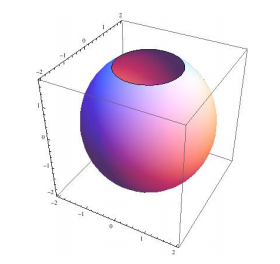
\includegraphics[height=7cm, width=10cm]{first.png}
      \end{center}

      Consider also the vector field:

      $$\mathbf{F}=zx \hat{x}+zy \hat{y}+z^2 \hat{z}$$
      \begin{enumerate}
        \item Calculate $\overrightarrow{\nabla} \times \mathbf{F}$.

          \textcolor{hwColor}{
            $
              \overrightarrow{\nabla} \times \mathbf{F}=\begin{vmatrix}
                \hat{i} & \hat{j} & \hat{k} \\
                \\
                \dfrac{\partial}{\partial x} & \dfrac{\partial}{\partial y} & \dfrac{\partial}{\partial z} \\
                \\
                zx & zy & z^2
              \end{vmatrix}=\left[\dfrac{\partial}{\partial y}z^2-\dfrac{\partial}{\partial z}zy\right]\hat{i}-\left[\dfrac{\partial}{\partial x}z^2-\dfrac{\partial}{\partial z}zx\right]\hat{j}+\left[\dfrac{\partial}{\partial x} zy-\dfrac{\partial}{\partial y}zx\right]\hat{k} \\
              \\
              \\
              \therefore \overrightarrow{\nabla} \times \mathbf{F}=-y \hat{i}+x\hat{j}
            $
          }

        \pagebreak
        
        \item Calculate the path integral $I=\oint_C \mathbf{F} ~ . ~ ds$ using Stokes theorem and the surface $\Sigma$.
        Consider the vector normal to $\Sigma$ to be oriented outwards.

          \textcolor{hwColor}{
            Since we are given a line integral and told to use Stokes' theorem, we need to compute a surface integral. \\ \\
            Stokes' theorem is a generalization of Green's theorem. This theorem is used when a curve is not on a plane. \\
            \\
            $
              \oint_C \overrightarrow{\mathbf{F}}.d\overrightarrow{s}=\iint_S ~ curl ~ \overrightarrow{\mathbf{F}}.d\overrightarrow{S}=\iint_S ~ (curl ~ \overrightarrow{\mathbf{F}}.\hat{n}) ~ ds \\
              \\
              curl ~ \overrightarrow{\mathbf{F}}=\overrightarrow{\nabla} \times \overrightarrow{\mathbf{F}}=-y \hat{i}+x\hat{j} \\
              \\
            $
            The sphere and the plane $z=\sqrt{3}$ intersect on a circle: \\
            \\
            $x^2+y^2+(\sqrt{3})^2=4 ~~ \Rightarrow ~~ x^2+y^2=1$ \\ \\
            By parameterizing it we have the following: \\
            \\
            $
              \begin{cases}
                x=rcos(\theta) \\
                y=rsin(\theta) \\
                z=1
              \end{cases} \\ \\
              \overrightarrow{s}(r,\theta)=rcos(\theta)\hat{i}+rsin(\theta)\hat{j}+\hat{k} \\
              \\
              \hat{n}ds=d\overrightarrow{\mathbf{S}}=(\overrightarrow{s_r} \times \overrightarrow{s_\theta}) d\theta dr \\
              \\
              \\
              \overrightarrow{s_r} \times \overrightarrow{s_\theta}=\begin{vmatrix}
                \hat{i} & \hat{j} & \hat{k} \\
                \\
                cos(\theta) & sin(\theta) & 0 \\
                \\
                -rsin(\theta) & rcos(\theta) & 0
              \end{vmatrix}=\hat{i}(0-0)-\hat{j}(0-0)+\hat{k}(r cos^2(\theta)+rsin^2(\theta))=\hat{k} \\
              \\
              \\
              \bigints_{r=0}^{r=1} \bigints_{\theta=0}^{\theta=2 \pi} \overrightarrow{\nabla} \times \overrightarrow{\mathbf{F}}.\hat{n}ds=\bigints_{r=0}^{r=1} \bigints_{\theta=0}^{\theta=2 \pi} (-y \hat{i}+x\hat{j}).(\hat{k}) ~ d\theta dr=0 \\
              \\
              \\
              \therefore \oint_C \overrightarrow{\mathbf{F}}.d\overrightarrow{s}=\iint_S ~ curl ~ \overrightarrow{\mathbf{F}}.d\overrightarrow{S}=0
            $
          }

      \end{enumerate}

    \pagebreak

    \item Consider the vector field $\mathbf{F}=(z+y) \hat{x}+z\hat{y}+(z+x)\hat{z}$. Consider also a frustum of cone, defined as:
    $$\begin{cases}
      z^2=x^2+y+2 \\
      1\leq z \leq 4.
    \end{cases}$$ 
    (see figure). Let us call $V$ the volume of this solid. Also, let $S$ be the closed surface enclosing the volume:
    $S=S_1\bigcup S_2 \bigcup S_3$, where $S_1$ is the flat bottom $(z=1)$, $S_2$ is the curved surface, and $S_3$ is the flat top $(z=4)$.
    \begin{enumerate}
      \item Calculate the flux $\Phi=\bigints_S \mathbf{F} ~ . ~ d\mathbf{S}$ using the appropriate boundary theorem (Gauss’
      theorem or Stokes theorem? Think carefully). [Hint: use cylindrical coordinates]
      
      \item Find the unit vector orthogonal to the surface $S_2$ and pointing out of the volume $V$. 
    \end{enumerate}

    \begin{center}
      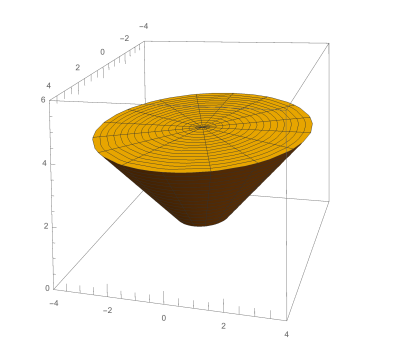
\includegraphics[height=7cm, width=10cm]{second.png}
    \end{center}
  \end{enumerate}

\end{document}
